\section{Implementation and Evaluation}
\label{sec:analysis}

The keyword solution and modifications to fission as described in subsections~\ref{sec:desugar} and~\ref{sec:fission} were implemented into the StreamIt compiler.  The sample benchmarks in Figure~\ref{fig:theo-speedups} were rewritten to use the {\tt iter()} keyword, allowing the compiler to expose data parallelism in its stream graph.  We use an evaluation architecture composed of 4 octal-core 2.00 GHz Intel Xeon x7550 processors, each with 18 MB L3 caches.  The architecture has 128 GB of available memory.


% The introduction of this iteration field creates state in the provided
% filter.  For future operations, the compiler does not consider this
% iteration field as part of the state of filter.  Future processes will
% maintain this inherent state without the downsides of explicitly
% introduced state.

% It is important to note, these filters are not classified as stateful
% to the user, even though the filter is actually stateful on the
% iteration count after the desugaring process.  In classifying filters
% as stateful, the user is made aware of where data parallelism may be
% inhibited.  Iteration filters will not inhibit data parallelism
% because its state is identifiable to the compiler during the fission
% process.



\subsection{FIRBankPipeline}
\begin{figure}[t]
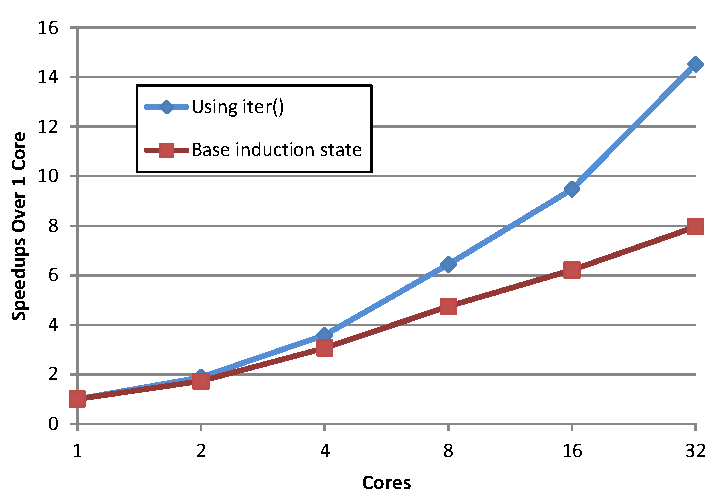
\includegraphics[width=3.3in]{figures/firbank-results.pdf}
\caption{Speedups for FIRBankPipeline, with and without induction variable state.  \protect\label{fig:firbank-results}}
\end{figure}

FIRBankPipeline contains one filter that uses induction variable state with 3.94\% of program's work.  This filter, Multiply, maintains induction state in an index that traces through the rows of a two dimensional array.  Each invocation performs complex multiplication on the stream input values and the array elements of that specified row.  

After removing the induction variable state, the compiler chooses to vertically fuse down the FIRBankPipeline program to a single filter.  Before the transformation, this is not done because of the induction variable state.  If the filter were fused down with the rest of the program, the end result would have been stateful, thus inhibiting data parallelism opportunities.  After removing this state, the program is stateless and can be fused and fissed to expose data parallelism.


Figure~\ref{fig:firbank-results} indicates the speedups over 1 core for both induction state and iteration keyword implementations.  Between the two implementations, there is 1.36X speedup on 8 cores, 1.58X speedup on 16 cores, and 1.83X speedup on 32 cores for the iteration keyword implementation.  This abides fairly closely with the model as described in Section ~\ref{sec:model-analysis}.  